\section{General Overview}
\label{sec: general_overview}

The design of the user interfaces (UI) for the S\&C platform plays an important role in ensuring an engaging user experience. In the following section, through the use of possible UI interfaces, a comprehensive overview of the platform and its functionalities will be given, highlighting the principles and features that make the platform intuitive and accessible for its diverse user base.

The UI features a clean and consistent layout, obtained with uniform visual elements across pages and intuitive icons and labels, ensuring users can quickly find what they need and understand differences between each section.

UI interfaces are not provided for every possible page described in the RASD \& DD documents, but only for the main pages which include the majority of the functionalities. Further interfaces can be made following the style provided in these layouts. Design choices, colors, fonts, and other elements can be modified accordingly in order to follow strategic business decisions to better engage the users.

Each webpage shown is responsive and adapts to all types of devices.

\newpage

\section{User Interfaces Layouts}
\label{sec: ui_layouts}

\subsection{Home Page}
\label{subsec: home_page}

\begin{figure} [H]
    \begin{center}
        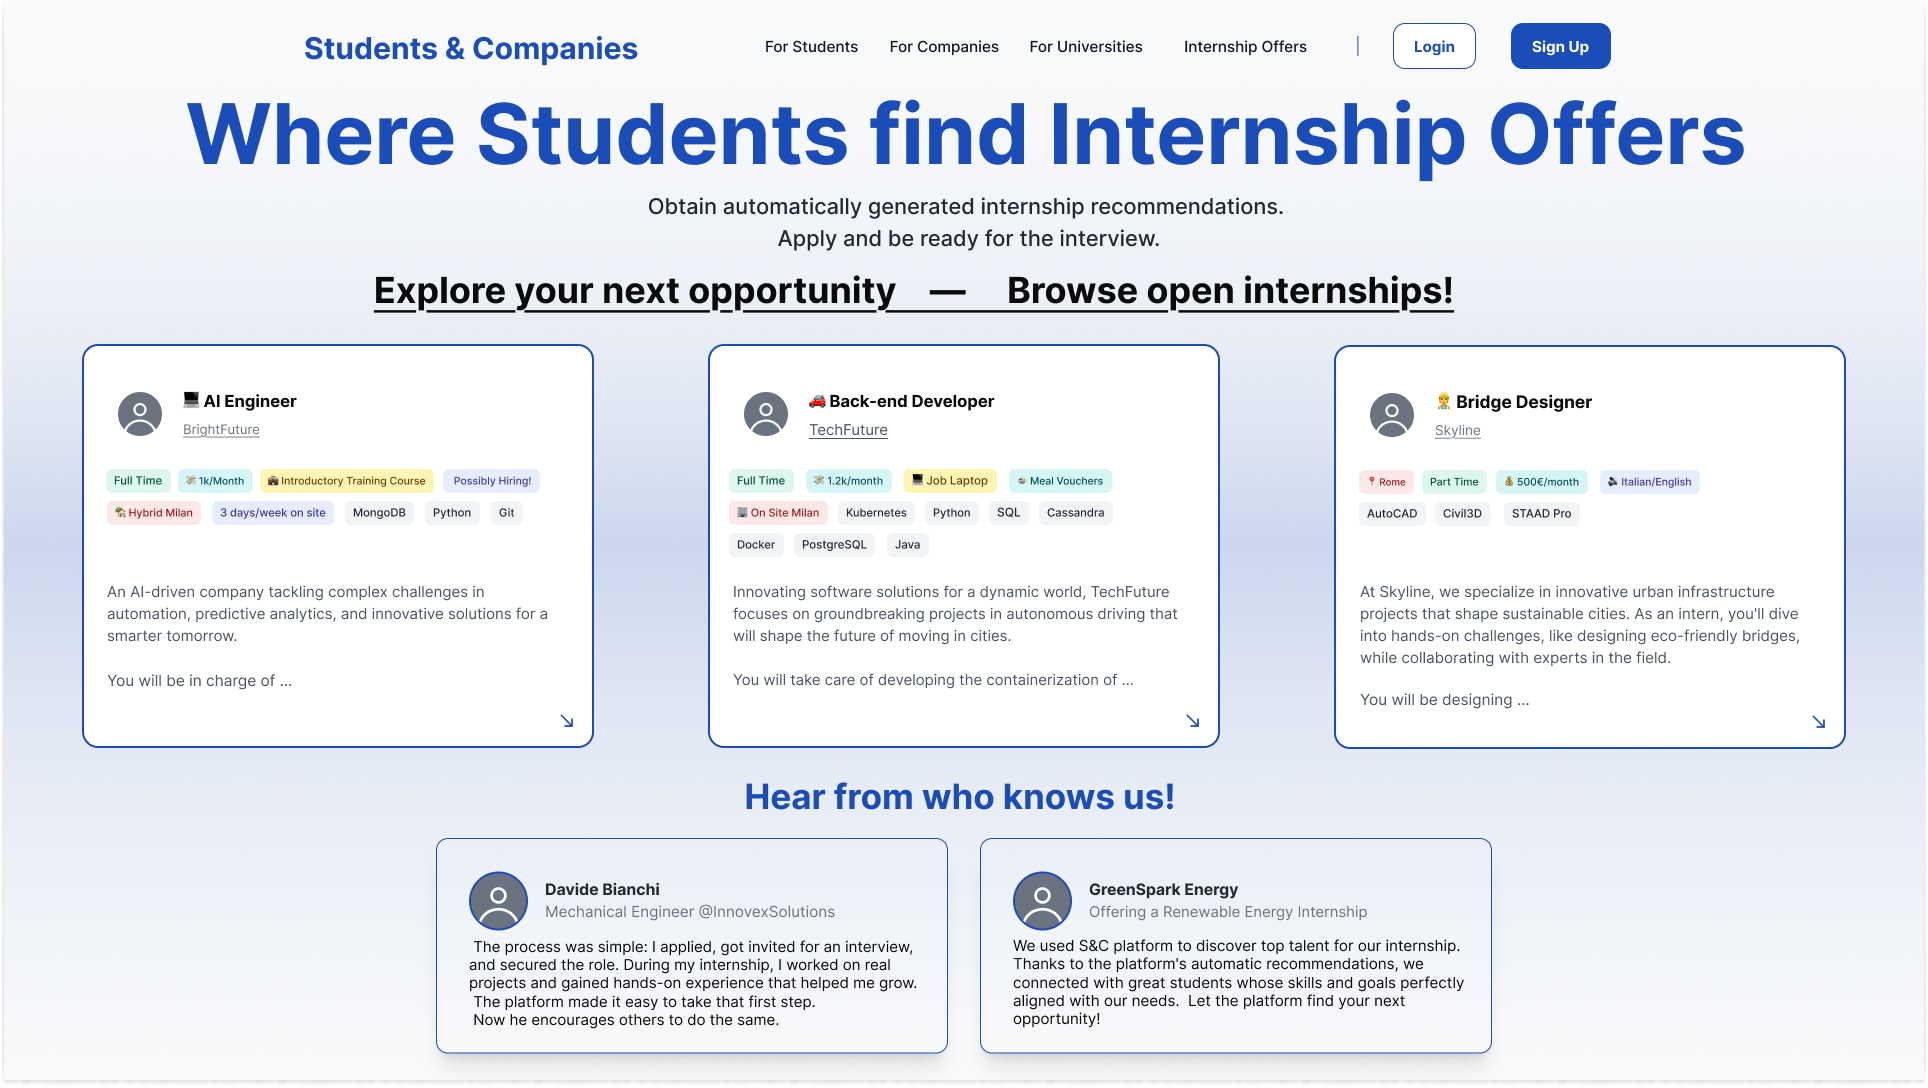
\includegraphics[width=0.9\linewidth]{LaTeXCode/images/UI/Homepage - Student.png}
        \caption{Landing Page of the WebApp}
        \label{fig: homepage}
    \end{center}
\end{figure}

The Home Page of S\&C is a multiple entry point for all the user groups. Its purpose is to guide students, companies, and universities to tailored content.
The navigation bar contains links to "For Students", "For Companies", "For Universities", which redirects to custom landing pages. In this case, the page displayed is specifically made for students.
The "Internship Offers" redirects to a browse-only carousel of internship offers, without any additional functionality prior to be registered.
The middle section displays some of the active internship opportunities in an interactive grid layout that can be manually moved by the user or automatically updates the showcased content after a certain time.
A testimonials section features true stories to build trust and credibility.
The page can also be extended vertically and made scrollable, to include more content and optionally a footer.

\subsection{Sign Up Page}
\label{subsec: sign_up_page}

\begin{figure} [H]
    \begin{center}
        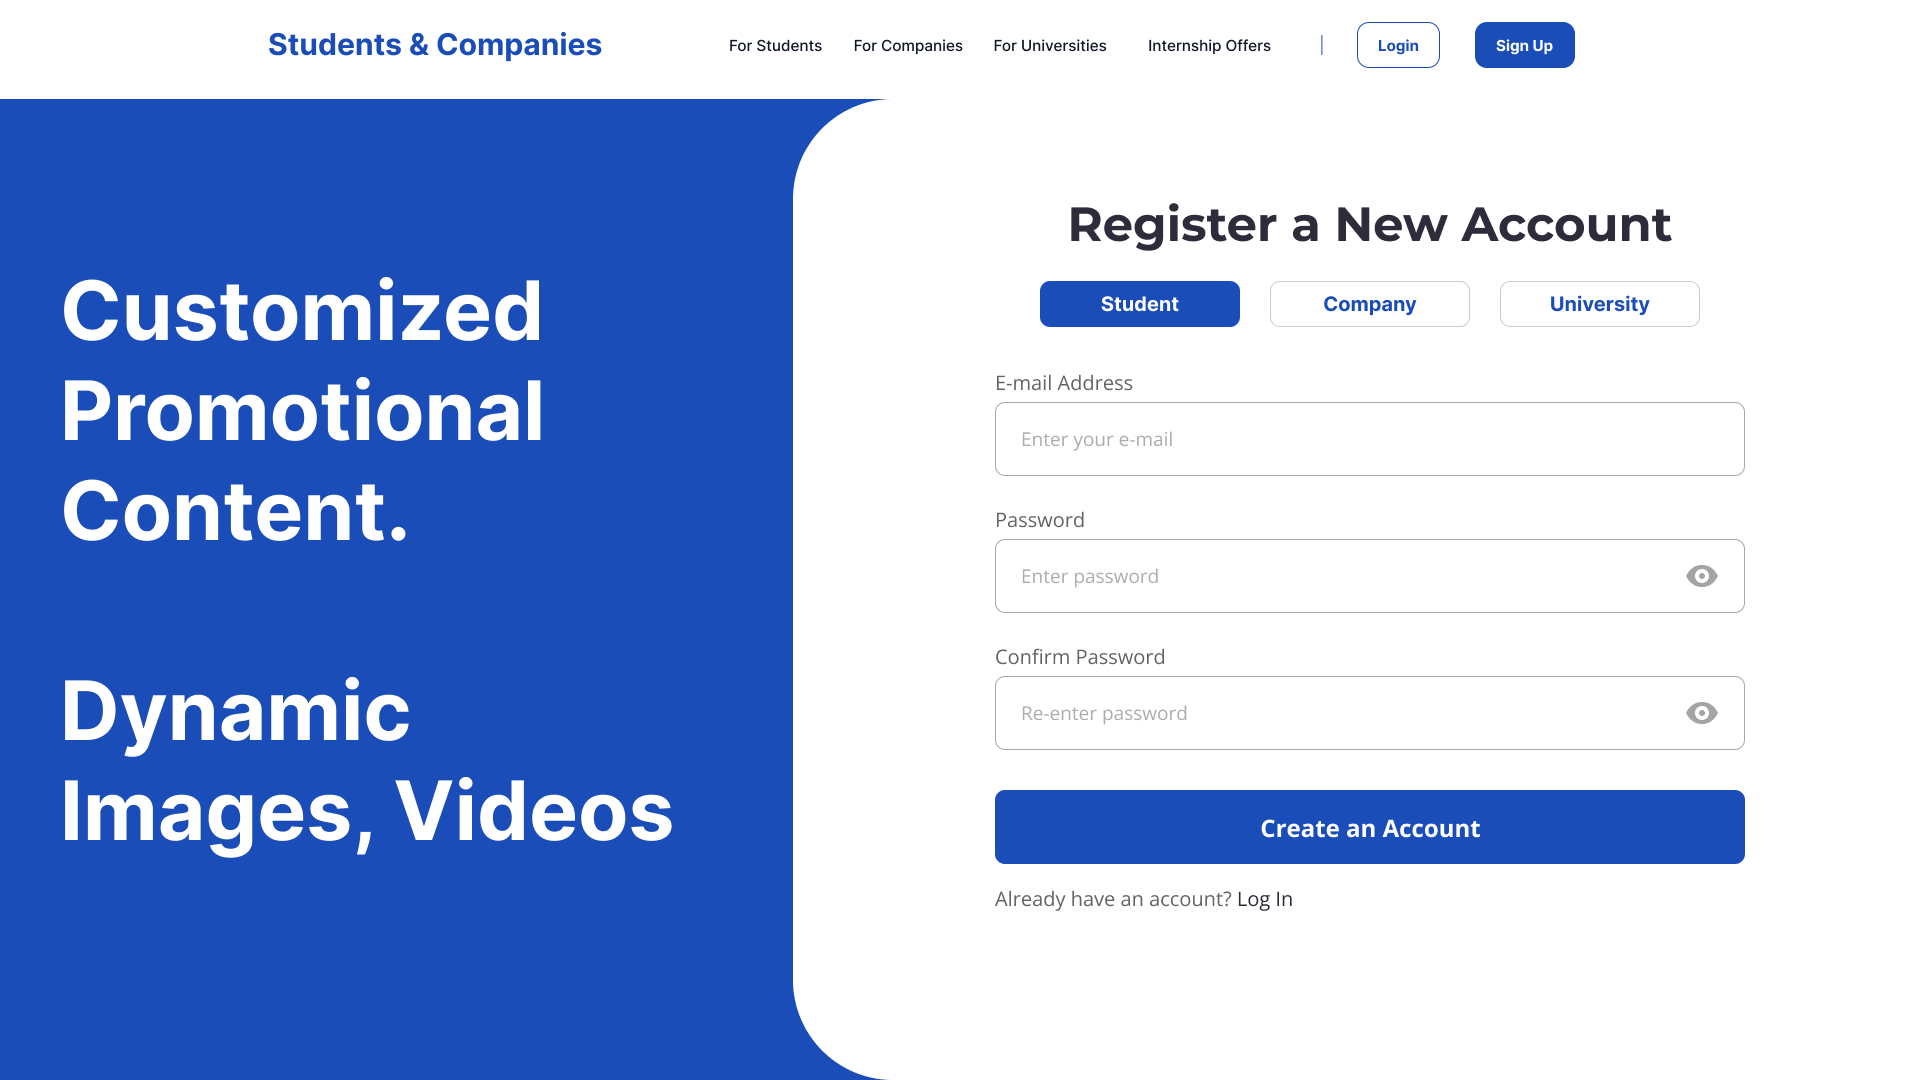
\includegraphics[width=0.9\linewidth]{LaTeXCode/images/UI/Sign Up - Unified Version.png}
        \caption{Sign Up - Initial Step}
        \label{fig: sign_up_unified}
    \end{center}
\end{figure}

The sign up page contains the initial step of the registration processes for all user groups. Additional information required to customize each profile will be collected in a subsequent form, accessible after the link in the confirmation email is accepted.
The navigation bar from the landing page remains consistently visible throughout the sign up process.

\subsection{Student Dashboard}
\label{subsec: student_dashboard}

The student dashboard contains all functionalities available to students. It is divided into three distinct views, accessible via a dropdown menu integrated into the navbar, only visible once a student is logged in.

\begin{figure} [H]
    \begin{center}
        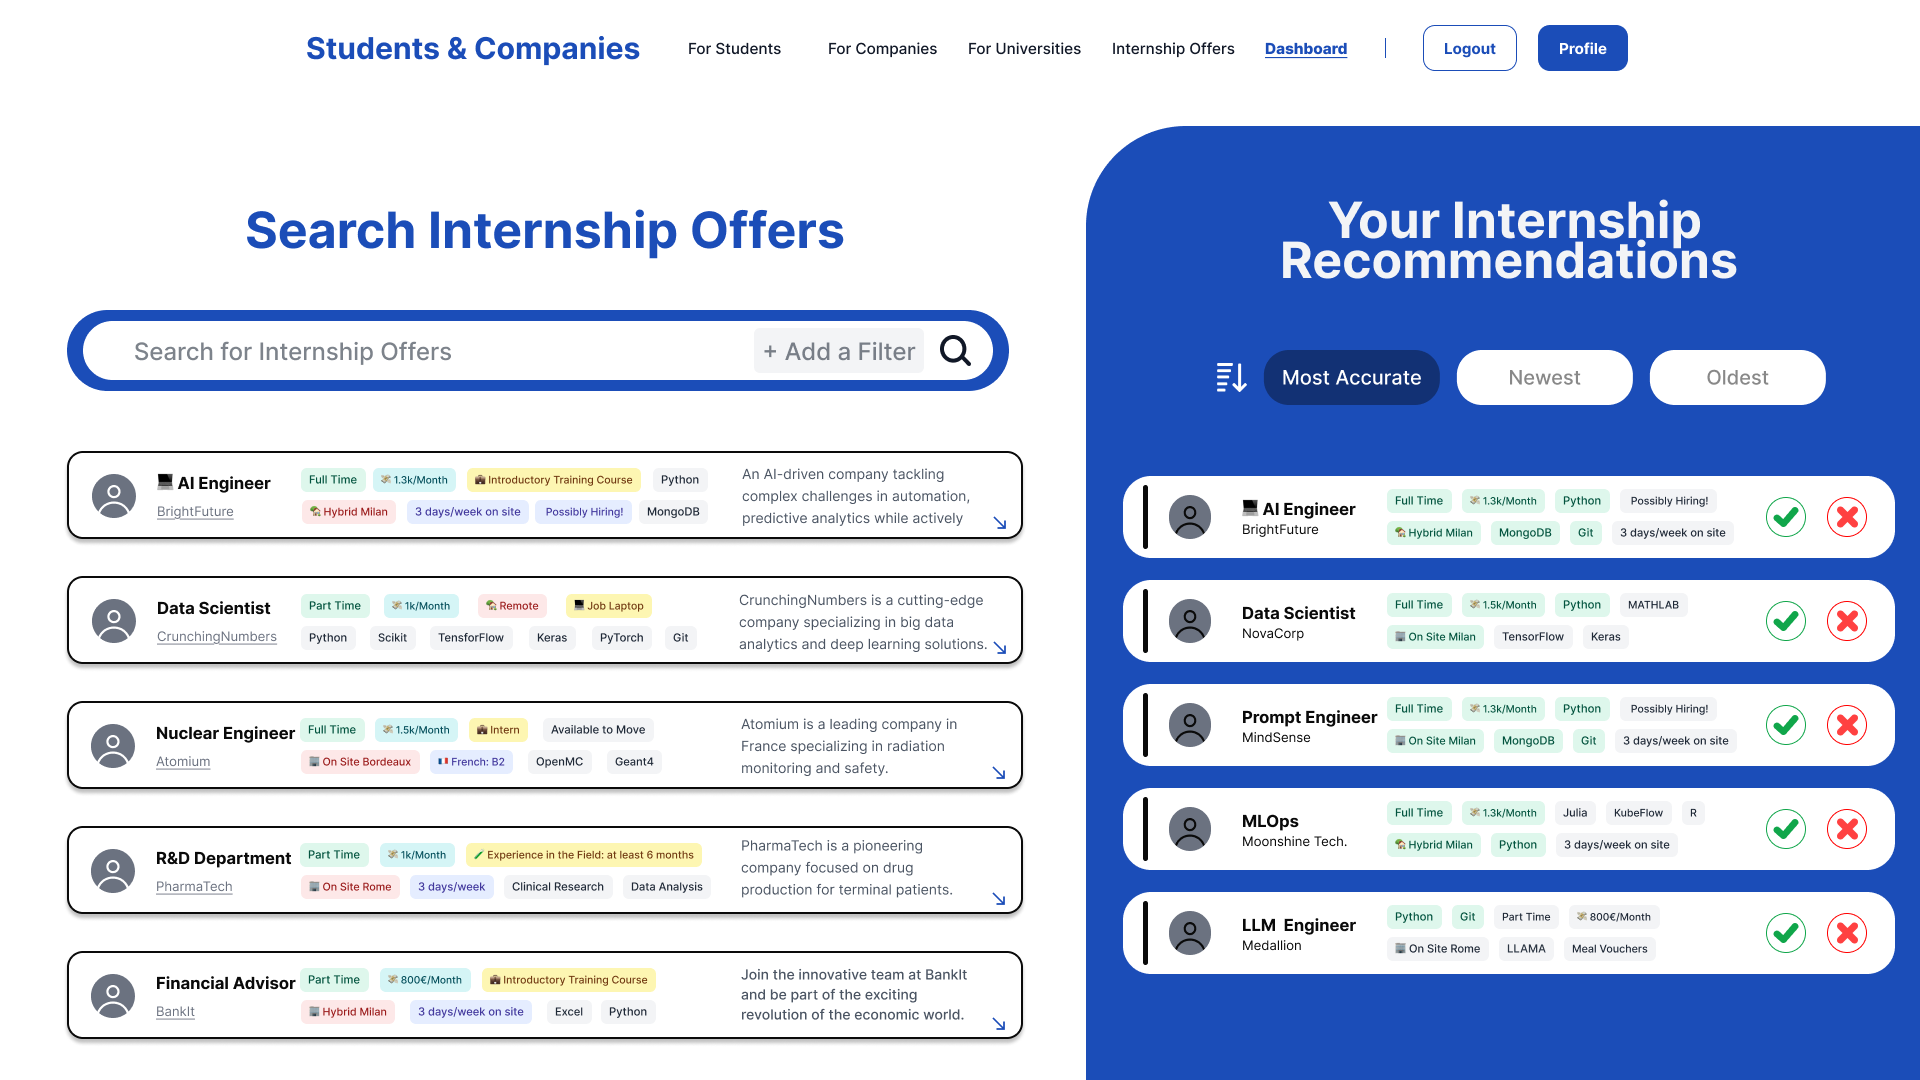
\includegraphics[width=0.9\linewidth]{LaTeXCode/images/UI/Student Dashboard - Main View.png}
        \caption{Student Dashboard - Main View}
        \label{fig: dashboard_student_main}
    \end{center}
\end{figure}

The main view, displayed by default whenever a student is redirected to the dashboard, is made by two sections: Search Internship Offers and Your Internship Recommendations.

On the left, the search functionality allows students to explore internship offers using a text-based search bar. The search can be further refined with predefined filters, such as keywords found in posted internship descriptions. If no input is provided, the system displays a random selection of internship offers. After initiating a search, the results appear in a vertical list layout. Each internship offer is an interactive element that opens a modal to display detailed information and includes the option to apply directly.

On the right, the Recommendations section shows the internship recommendations automatically generated by the system. Students can choose to accept or decline these recommendations and sort them based on predefined criteria, as indicated by the three intuitive sorting buttons. Each recommendation is interactive, allowing students to view offer details via a modal. 
As previously detailed in the document, students can apply directly through the internship offers or the recommendations with identical technical functionality.

Both sections are dynamic and adapt in real-time to user interactions.

\begin{figure} [H]
    \begin{center}
        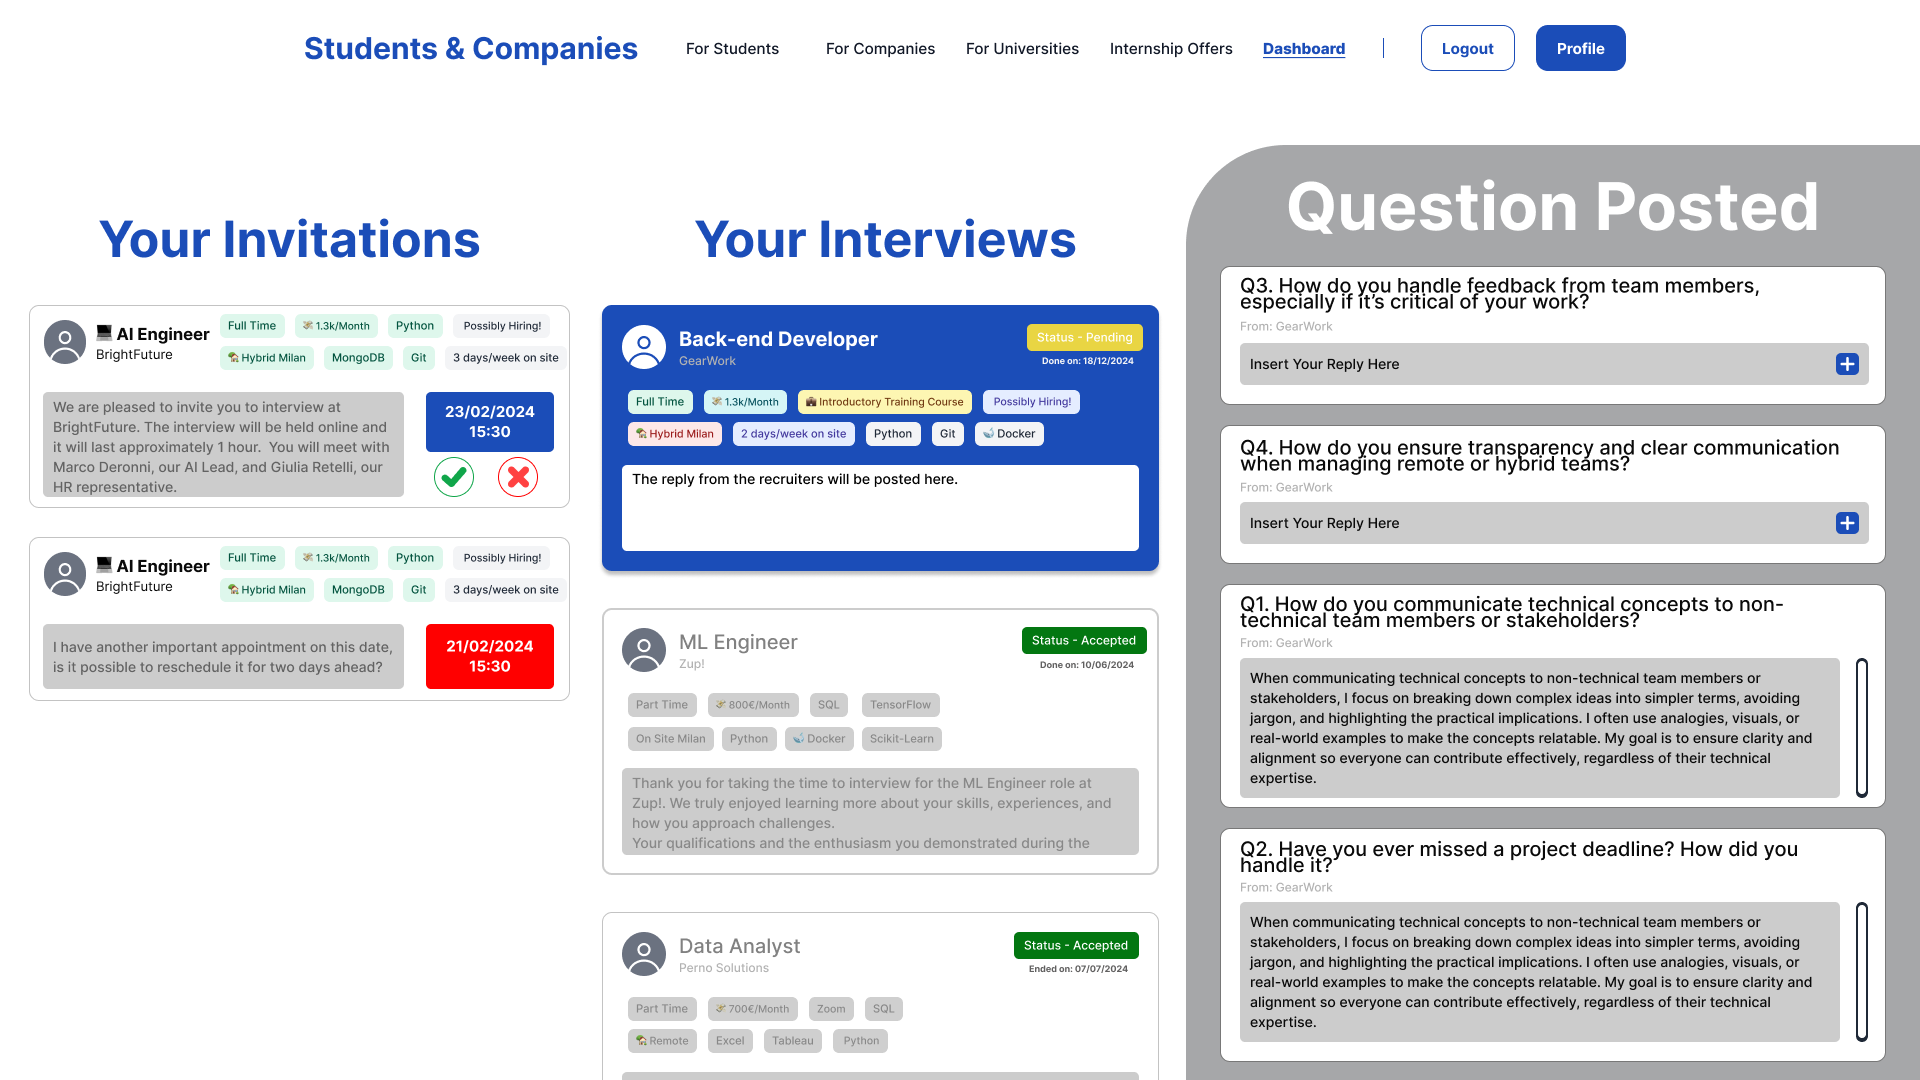
\includegraphics[width=0.9\linewidth]{LaTeXCode/images/UI/Student Dashboard - Second View.png}
        \caption{Student Dashboard - Second View}
        \label{fig: dashboard_student_second}
    \end{center}
\end{figure}

The second view, accessible through the drop-down menu, contains all the functionalities related to interviews and is divided into three sections: Your Invitations, Your Interviews, and a Message Board for questions related to the internships you have applied for.

On the left side, the Your Invitations section displays all pending, accepted, and refused interview invitations for internship offers where the interview process is still ongoing. Invitations are sorted chronologically, with the most recent ones appearing at the top. If a student declines an invitation, a modal will appear, asking to provide a reason or message to the hiring company.

The middle section, Your Interviews, lists all completed interviews. Each entry includes a summary of the position applied for, the interview date, and the current status of the application. 
When the company ends the process, feedback from the recruiter is displayed within each interview entry. Similar to the Invitations section, interviews are organized chronologically from top to bottom.

On the right side, the Message Board displays questions posted by companies conducting interviews for the internships you’ve applied to. Unanswered questions are shown at the top, while those you’ve already responded to appear below. Since questions from different companies may appear in a mixed layout, each question identifies the company that posted it. Alternatively, a filtering option by company can be added to obtain a separated view for each company. Once a selection process is completed, associated questions are automatically removed from the board.

\begin{figure} [H]
    \begin{center}
        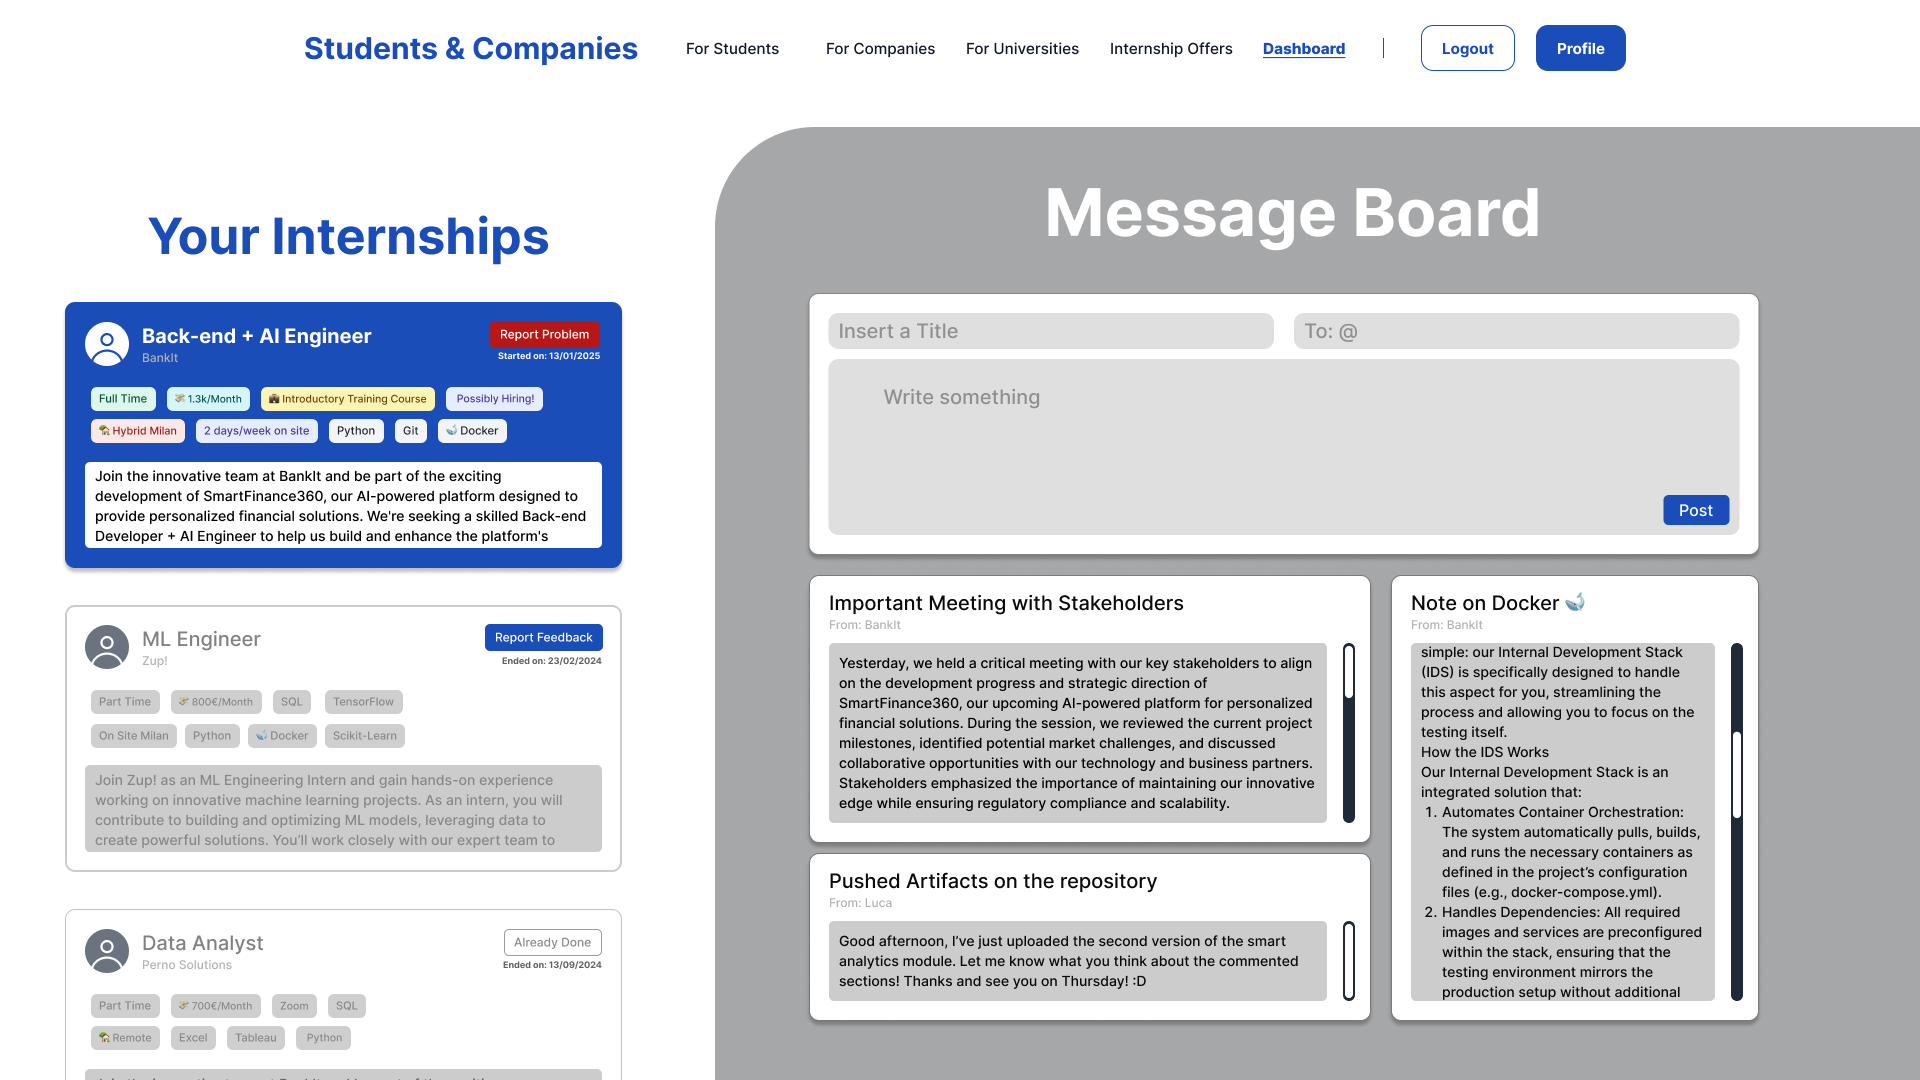
\includegraphics[width=0.9\linewidth]{LaTeXCode/images/UI/Student Dashboard - Third View.png}
        \caption{Student Dashboard - Third View}
        \label{fig: dashboard_student_third}
    \end{center}
\end{figure}

The third view, accessible through the dropdown menu, provides all functionalities related to ongoing and completed internships, organized into two sections: Your Internships and a Message Board for communication with the company.

On the left, the Your Internships section displays details of both ongoing and completed internships. Each ongoing internship includes a summary of the applied position, the starting date, and a "Report Problem" feature that initiates a process managed by the university to address issues. Completed internships are also listed here, with the option to provide feedback if it has not already been submitted. As in other sections, internships are sorted chronologically, with the most recent at the top.

On the right, the Message Board provides a dedicated space for displaying all communications between the student(s) and the company. At the top, students can post new messages, while previous messages are displayed below in chronological order. Older messages can be accessed by scrolling further down the section, ensuring all messages remain accessible.

\subsection{Profile Page - Student}
\label{subsec: profile_page_student}

\begin{figure} [H]
    \begin{center}
        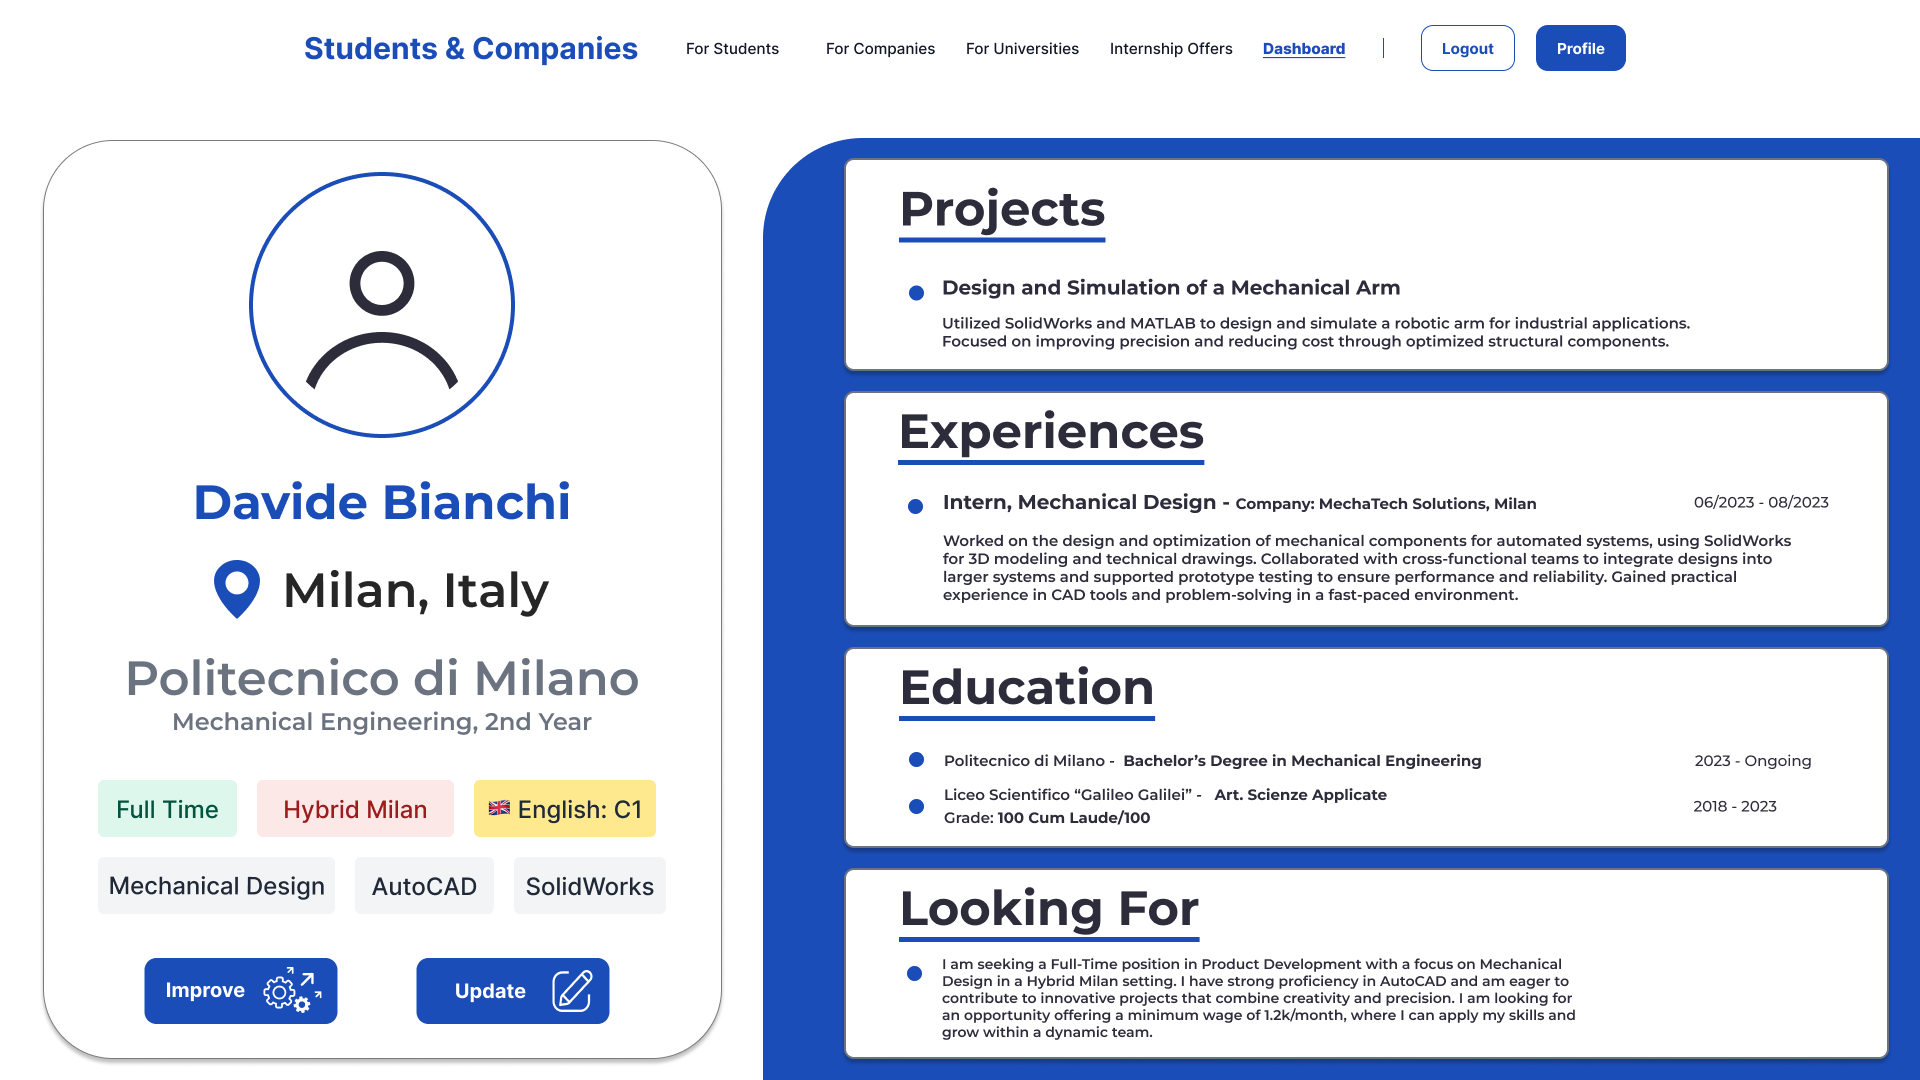
\includegraphics[width=0.9\linewidth]{LaTeXCode/images/UI/Student Dashboard - Profile.png}
        \caption{Profile Page - Student}
        \label{fig: profile_student}
    \end{center}
\end{figure}

The Profile page, accessible through the navigation bar, contains all information related to the student.

On the left, a summary of the student’s profile is displayed, highlighting the most relevant details along with a subset of keywords extracted from their complete profile. Below this summary, two key actions are available: Suggest Optimizations for a Student Profile, which provides recommendations to enhance the profile, and Update Profile, allowing students to edit their information.

On the right, the main subsections of the curriculum are presented. These sections are used to identify and extract keywords that define the student's keywords.

Other profile pages expected in the platform, for Company and University, are similar in the general layout and only differ in the content shown, and so for this reason their UI is not provided in this document.

\subsection{Company Dashboard}
\label{subsec: company_dashboard}

The company dashboard contains all functionalities available to companies. It is divided into three distinct views, accessible via a dropdown menu integrated into the navbar, only visible once a company is logged in.

\begin{figure} [H]
    \begin{center}
        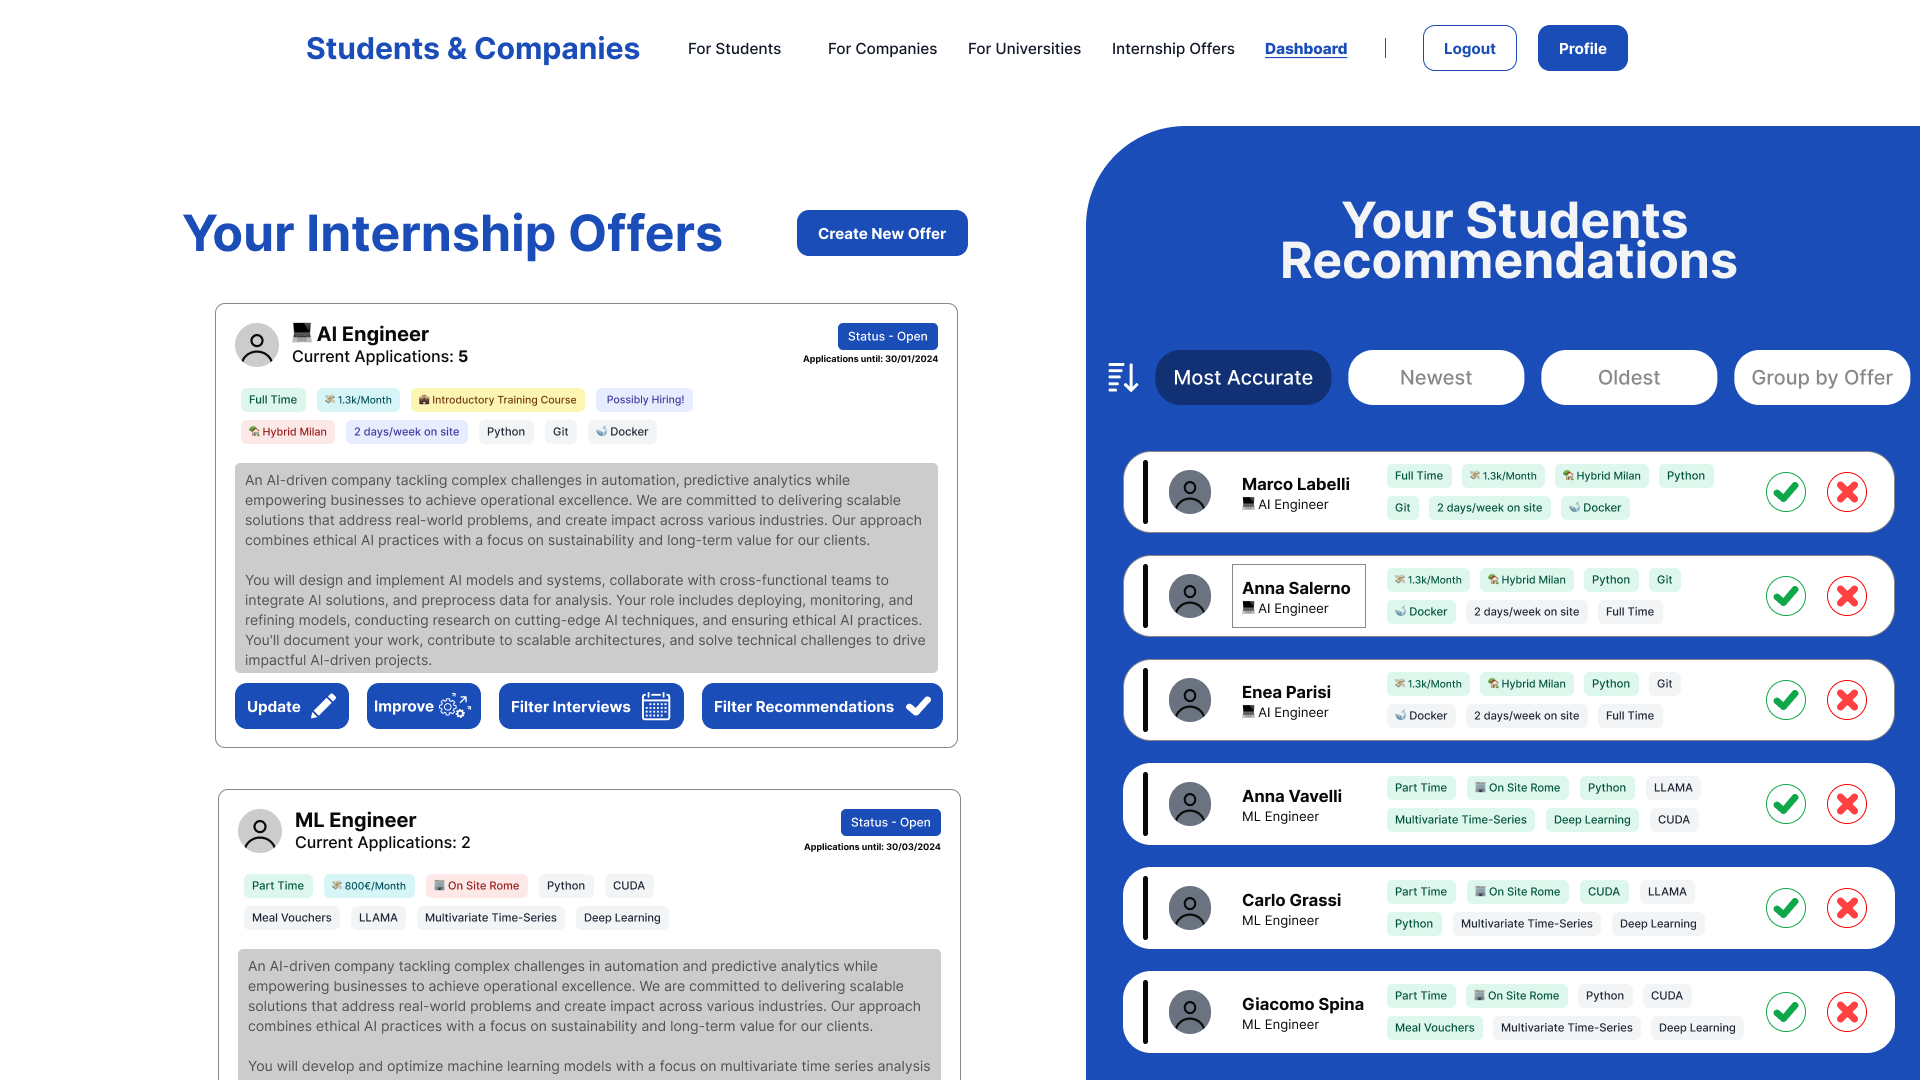
\includegraphics[width=0.9\linewidth]{LaTeXCode/images/UI/Company Dashboard - Main View.png}
        \caption{Company Dashboard - Main View}
        \label{fig: dashboard_company_main}
    \end{center}
\end{figure}

The main view, displayed by default whenever a company is redirected to the dashboard, is composed of two sections: Your Internship Offers and Your Students Recommendations.

On the left, all open internship offers are listed, displaying the description provided during posting and relevant keywords extracted from the description.
To perform the insertion of a new internship offer on the platform, companies can use the associated button, which opens a modal containing a form with all the required fields to be compiled.
Each internship is an interactive element that can be expanded into a modal for detailed visualization, including its description and a list of applicants. Below each internship, there are further options: one to edit the offer's details or eventually withdraw it and another to receive suggestions for improving its content. A Filter Interviews button allows navigation to the Interviews section of the dashboard, focusing exclusively on interviews and invitations for that specific offer. By default, the Interviews section displays invitations and interviews for all internships currently in the Selection phase. Additionally, a Filter Recommendations button performs a similar action, filtering the Recommendations section (on the right) to suggestions relevant to the selected internship.

On the right, the Recommendations section shows the student recommendations automatically generated by the system. Companies can accept or decline these recommendations and sort them using four intuitive sorting buttons. Each recommendation highlights the compatibility between internship offer keywords and student profiles. Recommendations are interactive, enabling companies to view detailed student profiles through a modal.

\begin{figure} [H]
    \begin{center}
        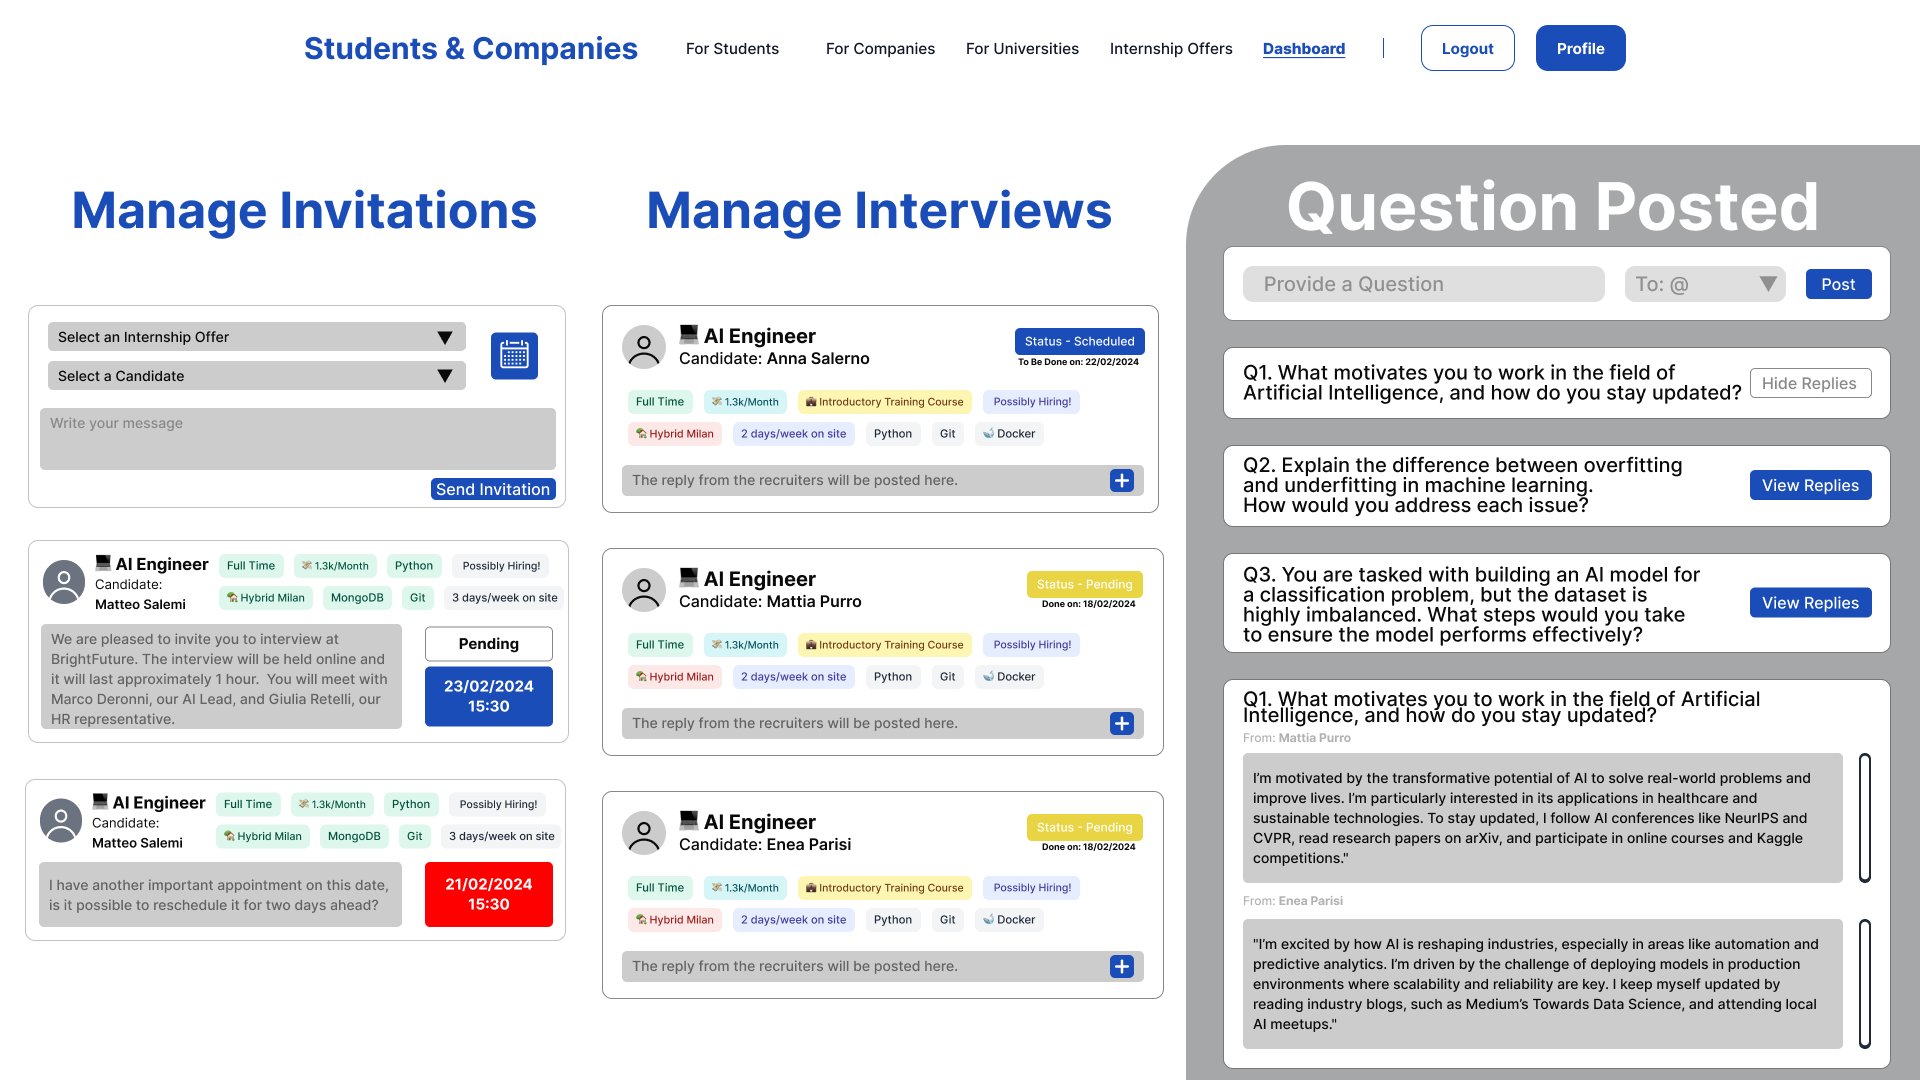
\includegraphics[width=0.9\linewidth]{LaTeXCode/images/UI/Company Dashboard - Second View.png}
        \caption{Company Dashboard - Second View}
        \label{fig: dashboard_company_second}
    \end{center}
\end{figure}

The second view, accessible via the drop-down menu or the previously mentioned shortcut, contains all functionalities related to interviews. It is divided into three sections: Manage Invitations, Manage Interviews, and a Message Board for providing questions to candidates during interviews.

On the left, companies can create new invitations by selecting the associated internship offer and choosing a candidate from a dropdown menu, specifying a proposed date and time, and providing a description. Below this, all refused and pending invitations are displayed, while accepted invitations automatically move to the middle section.

The middle section shows all scheduled interviews, sorted chronologically. Here, companies can provide feedback on each interview, which includes a status field that can be updated by clicking on it to finally accept or decline the candidate.

On the right, the Message Board allows companies to post new questions to candidates, selecting one or multiple candidates through a dropdown menu. Companies can also monitor replies to previous questions, with options to view or hide specific questions using dedicated buttons.

\begin{figure} [H]
    \begin{center}
        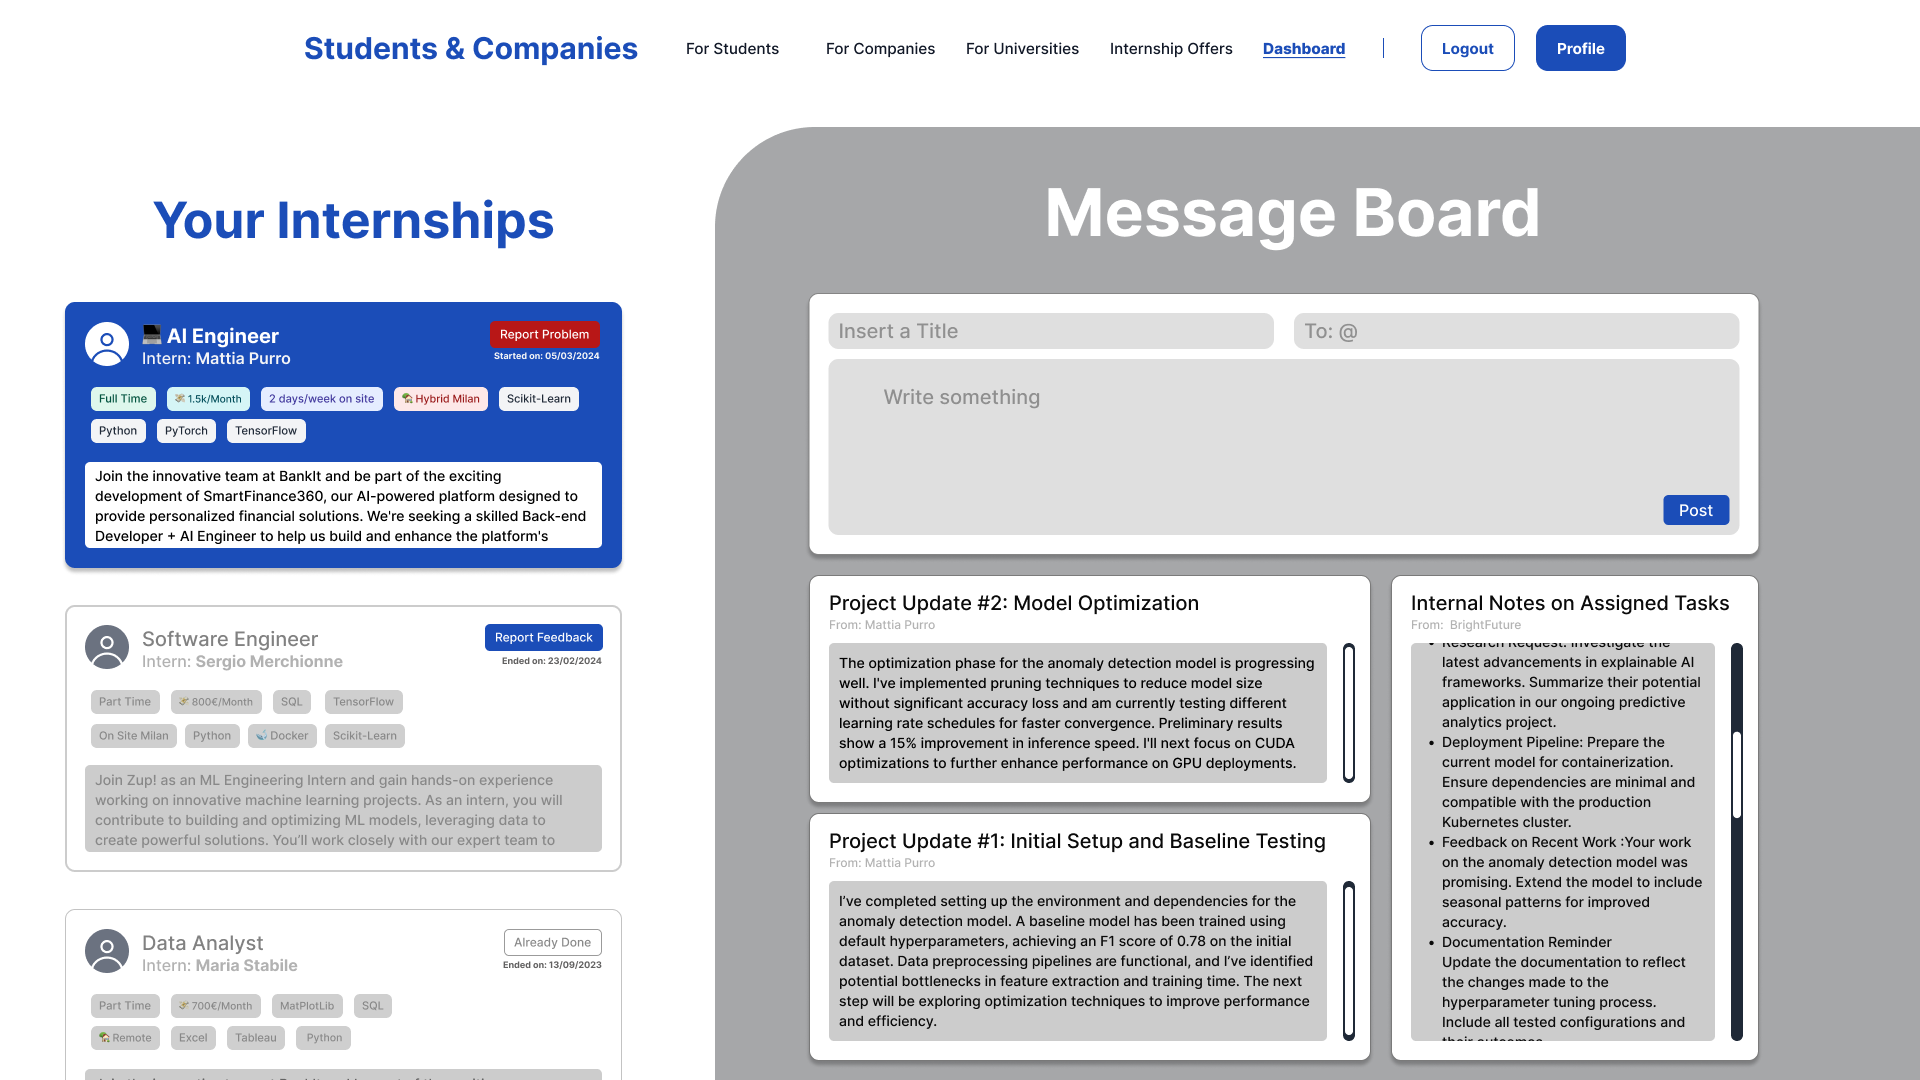
\includegraphics[width=0.9\linewidth]{LaTeXCode/images/UI/Company Dashboard - Third View.png}
        \caption{Company Dashboard - Third View}
        \label{fig: dashboard_company_third}
    \end{center}
\end{figure}

The third view, accessible through the dropdown menu, provides all functionalities related to ongoing and completed internships, organized into two sections: Your Internships and a Message Board for communication with the students.

On the left, the Your Internships section displays details of both ongoing and completed internships. Each ongoing internship includes a summary of the applied position, the starting date, and a "Report Problem" feature that initiates a process managed by the university to address issues. Completed internships are also listed here, with the option to provide feedback if it has not already been submitted. As in other sections, internships are sorted chronologically, with the most recent at the top.

On the right, the Message Board provides a dedicated space for displaying all communications between the company and the student(s). At the top, companies can post new messages, while previous messages are displayed below in chronological order. Older messages can be accessed by scrolling further down the section, ensuring all messages remains accessible.

\subsection{University Dashboard}
\label{subsec: university_dashboard}

The university dashboard contains all functionalities available to universities. It is composed by a minimal view, accessible via the dashboard link integrated into the navbar, only visible once a university is logged in.

\begin{figure} [H]
    \begin{center}
        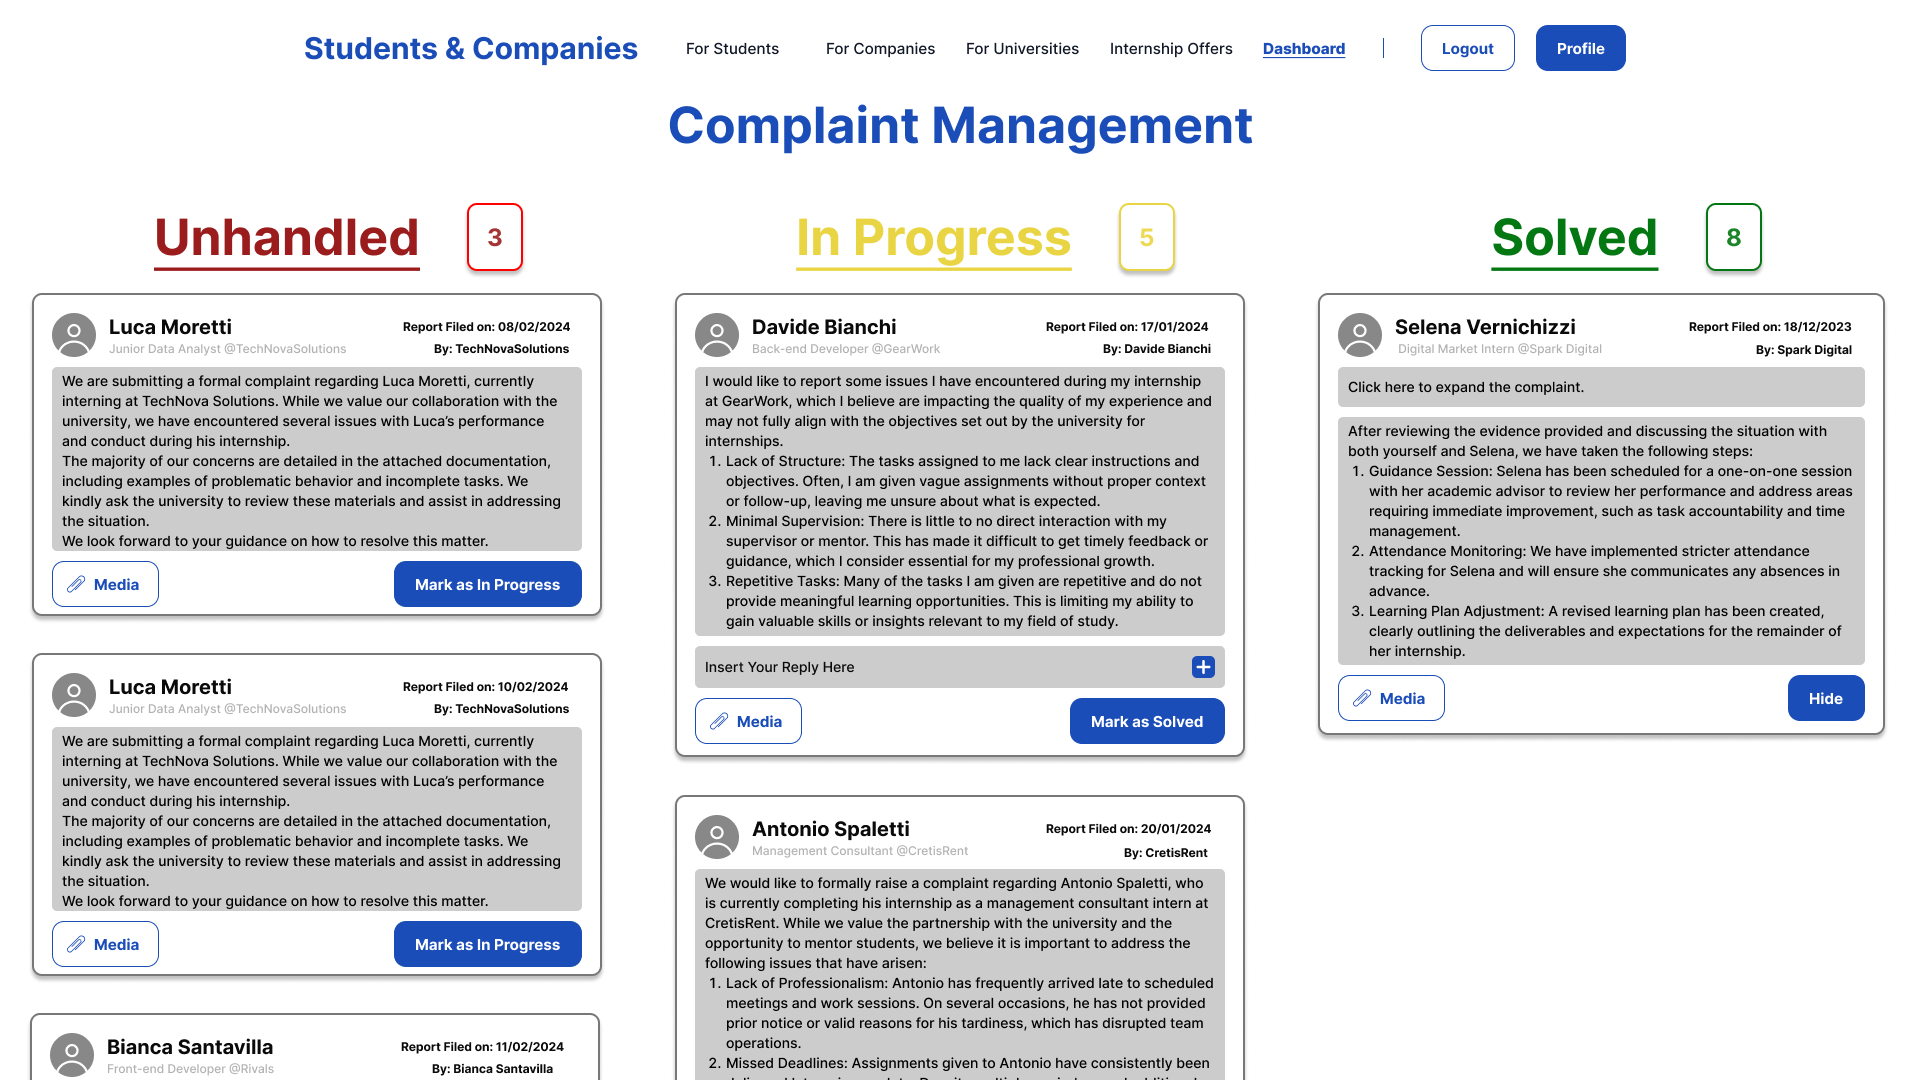
\includegraphics[width=0.9\linewidth]{LaTeXCode/images/UI/University Dashboard - Complaint Management View.png}
        \caption{University Dashboard - Complaint Management View}
        \label{fig: dashboard_university_complaint}
    \end{center}
\end{figure}

The default view, displayed whenever a university is redirected to the dashboard, consists of three sections that form the Complaint Management Dashboard. This dashboard enables the university to execute the "Handle Problems" functionality for their students.

The layout is intuitive, featuring a three-column pipeline that organizes complaints based on their status: Unhandled, In Progress, or Solved. Complaints are displayed in reverse chronological order within each column, with the oldest reports at the top and the newer ones below.

Each report includes comprehensive details about the student, their role, the date the report was filed, and the reporting party. A description of the issue is presented in a dedicated text section, and any attached media can be accessed by clicking the Media button.

When the status of a report changes, it automatically moves to the corresponding adjacent column. Once a report is marked as solved, the university has the option to hide it from the dashboard view to reduce clutter.

To improve focus, the university can hide any of the three columns by clicking the corresponding label. The remaining columns will dynamically adjust to occupy the available space equally.
